% !TeX root = paper.tex
\documentclass[a4paper,12pt]{article}

% Packages
\usepackage[utf8]{inputenc}     % For UTF-8 encoding
\usepackage{amsmath, amssymb}   % For math symbols
\usepackage{graphicx}           % For including graphics
\usepackage{geometry}           % For setting page margins
\usepackage[numbers]{natbib}             % For citations
\usepackage{hyperref}           % For clickable links in references
\usepackage{subcaption}         % For side by side subfigures
% Page layout
\geometry{margin=1in}           % Set margins to 1 inch

% Title section
\title{Tina Paper In Development}
\author{Your Name}
\date{\today}




\begin{document}

\maketitle

\begin{abstract}
    This is the abstract of your paper. Briefly describe the purpose of the research, the main results, and the conclusions.
\end{abstract}

\section{Introduction}
The study of tree rings has proven useful across multiple fields, proving to be a reliable subject for reconstructing past climates of regional and local environments, as well as a mechanism to understand tree growth response \citep{fritts_dendroclimatology_1971} \citep{williams_using_2010} \citep{guibal_dendrochronology_2021} \citep{sheppard_dendroclimatology_2010}.
To obtain these data from the tree rings, it is necessary to measure tree rings from a tree cookie or core. The first high precision tool for this purpose was a stage micrometer, involving a trained technician to incrementally shift a tree core under the objective of a microscope - informing a computer when a new ring is encountered \citep{robinson_microcomputer_nodate}.
While this method has very high precision, the data is only as accurate as the experience and knowledge of the technician at the time of recording \citep{levanic_atrics_2007}.
The desire to remove repetition of errors in sampling and sampling bias across to individual technicians led researchers to an alternative - image analysis. 

The first step in measuring tree ring width from images requires the digitization of the sample from one of two major methods.  
The original technique was as a flatbed scanner which can digitize the entire sample at once \citep{guay_new_1992}. 
With a top of the line scanner, like the Epson Perfection V850 Pro, it's possible to scan at maximum resolutions of 4800 dpi and scan an area of up to 8.5" x 11.7".
Analysis which relies on higher resolution larger samples require a different digitization approach. 

The second digitization model was introduced with ATRICS \citep{levanic_atrics_2007}. 
Rather than scanning a whole sample at once, a high resolution camera takes multiple images across the surface of the sample and uses image stitching software techniques to combine them into one ultra high resolution image \citep{muhlich_stitching_2022}.
Stitching multiple images into one mosaic has been applied in other fields such as mineralogy and cellular biology \citep{ro_image_2021,mohammadi_fast_2024}. 
This method requires either the camera objective to move relative to the sample, or the sample move underneath a stationary camera. 
For ATRICS and a more modern do-it-yourself alternative, CaptuRING, the sample is moved relative to the camera \citep{garcia-hidalgo_capturing_2022}. 
Gigapixel takes a different approach by moving the camera relative to the sample, allowing for multiple samples to be recorded in sequence. 
While these machines can all digitize cores, none have been shown to digitize cookies.

Tina was made to combine the defining features of the previously mentioned machines into one while making the project open-source and open-hardware. 
We designed Tina to digitize both cookies and cores, increase the maximum sample length, perform image stitching without operator intervention, all while minimizing cost. 
Successful functionality of this system is dependent on the major steps in tree cookie and core digitization to be automated. 
The only specialized piece of equipment needed to build Tina is a 3D printer, but the parts can be readily ordered through 3D print shops if preferred.
Excluding 3D printed parts, the total cost of the machine is approximately \$2,200 USD compared to the \$70,000 USD of the Gigapixel \citep{griffin_gigapixel_2021}.
The total cost of the machine is almost comparable in price or less to many professional camera and macro lens combinations.
Additional savings can also be had when factoring in the cost of a professional stitching software license such as PTGui. 

\section{Methods}

\subsection{System Overview} % this is so dry fix later

Tina can be thought of as a combination of multiple subsystems: the camera, computer, and gantry machine. 
Cartesian movement in the X, Y and Z directions is a result of two machine kits and a motor controller from OpenBuilds - the ACRO 1010, the NEMA 17 lead screw linear actuator, and the X32 Motor Controller running GRBL firmware. 
Building on top of kits allowed for quick assembly and prefabricated parts saving development time. 
To fit on the build plates of the ACRO system, we made an adapter to connect the linear actuator to the X and Y axis, thus creating motion in the Z axis.
On the linear actuator's build plate, adapters were made to hold a 12MP Raspberry Pi HQ Camera equipped with a SEEED studio microscope lens connected to an NVIDIA Jetson Orin Nano (Jetson) through a CSI cable.
By choosing this combination, we were able to reduce the weight and cost of the camera significantly - trickling the budget into an efficient computer which can handle intensive image processing. 
The Jetson is a powerful edge computer which drives a computer monitor for a GUI, sends commands to the motor controller to move the machine, runs image processing calculations for automatic control, and performs calculations to stitch individual images into one mosaic. 
Despite the weight reductions, torsion on the gantry arm still resulted in a non-zero torsional deflection. A torsion correcting adapter was designed to counteract this rotation and level the lens.

\subsection{Sample Digitization} % Methods
The subsystems can be best understood by following the process from sample setup through the computing process to create the stitched image. 

To achieve this with a fixed focus camera, the samples must be nearly orthogonal to the camera lens. Misalignments between the sample and lens up to 10 degrees can be corrected by using the 3D printed sample levelling table we designed (See Figure \ref{fig:ideal_levelling}).
Once the sample is level, the operator interacts with the machine through the GUI to navigate the camera to the center of the sample, and focuses the preview image to be sharp. The height and width dimensions are then entered in the GUI
to be saved along with the detected center coordinate of the sample. This procedure can be repeated to create a queue of samples to digitize.

The height, width, identifiers, and centering of the sample is sufficient information to digitize.

\begin{figure}
    \centering
    \begin{subfigure}{.5\textwidth}
      \centering
      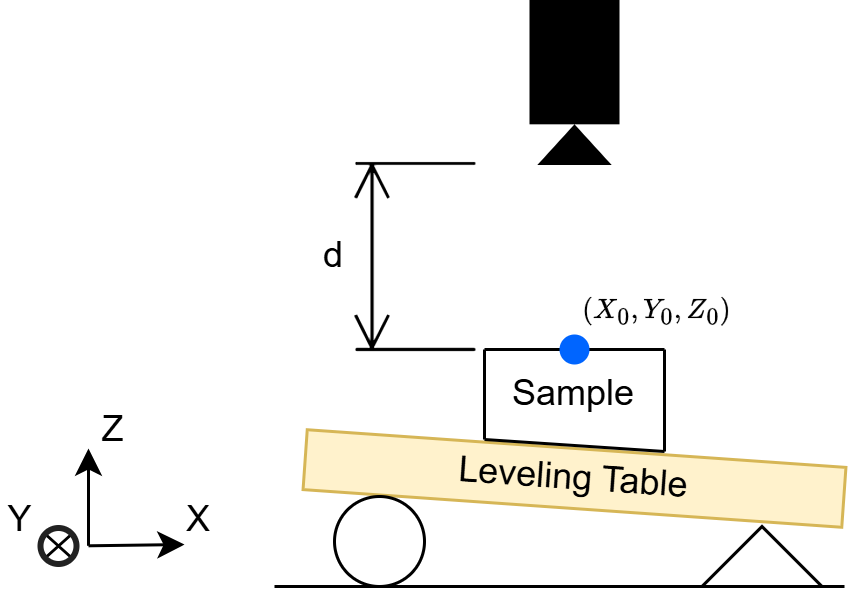
\includegraphics[height=0.5\linewidth]{../diagrams/sample_setup_ideal.png}
      \caption{Ideal sample leveling}
      \label{fig:ideal_levelling}
    \end{subfigure}%
    \begin{subfigure}{.5\textwidth}
      \centering
      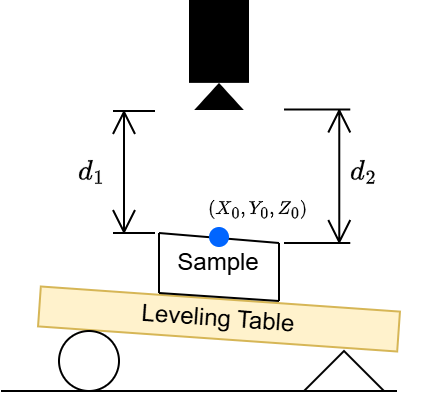
\includegraphics[height=0.5\linewidth]{../diagrams/sample_setup_realistic.png}
      \caption{Realistic sample leveling}
      \label{fig:realistic_levelling}
    \end{subfigure}
    \caption{Side view of the camera and sample on top of a leveling table. The ideal sample leveling shows a uniform distance d at all $(X,Y)$ coordinates on the sample. This is impossible to achieve in reality, the true sample leveling has a non uniform distance at unique $(X_i, Y_i)$.}
    \label{fig:sample_levelling}
\end{figure}


\subsection{Image Capturing}
Once prompted the system begins to exhaustively traverse the surface area of the sample. 
The goal of this traversal is to obtain in-focus images that have a region of overlap with all its neighbors - the basis of image stitching. 
Digitizing cores can often be done without needing to traverse in both the X and Y axis as the field of view in an image can capture the core's entire axial diameter in its field of view when moving along the core's length. % confusing wording fix later
Spanning the surface area of a cookie is more complicated as it needs move in both the X and Y axis (see Figure).

By centering the design around a fixed focus camera and lens, it is necessary to implement some sense of automatic control to focus the images. 
In this system, the only way to control focus is by changing the lens's distance to the sample. 
And with the microscope lens, the depth of field of the image is so sensitive that a perturbation of less half of a millimeter can move an entire image out of focus.
Solving this in a time efficient manner involves two stages. 
The first stage takes advantage of the requirement to navigate and focus the camera to the center of the sample.
This allows the initial $Z_0$ value from $(X_0, Y_0, Z_0)$ to be an informed initial guess as to what value would have an in focus image across the entire surface. 
Sample surface misalignment and a non flat sample (bumpy) surfaces require more than one image to be taken at each image $(X, Y)$. 
From the first $(X_0, Y_0)$ coordinate captured, 11 images are taken at different $Z$ values in $\boldsymbol{Z_{\text{focus}}}$. 
So long as $Z_{sample}$ is within this set, an in focus image exists.

\[
Z_{sample} \in
\boldsymbol{Z_{\text{focus}}} = 
Z_0 + 
\begin{bmatrix}
-0.5 \\
-0.4 \\
\vdots \\
0.4 \\
0.5 \\
\end{bmatrix}
\exists 
Z_{focused}
\] % unsure if this makes sense

Beginning at 0.5 mm above $Z_0$ and the last image finishing at 0.5 mm below $Z_0$.
To reduce motion blur in the images, this $\boldsymbol{Z_{\text{focus}}}$ is traversed at constant velocity and images are captured without stopping. 
The 11 images then have their normalized variance, $NV$, calculated in a separate thread to measure the image sharpness \citep{sampat_extensive_2014}.
The image with the maximum score is saved while the rest are deleted from storage.

\[
    i_{\max} = \arg\max_{i} NV(image(\boldsymbol{{Z_\text{focus}})})
\]
    
This focusing procedure works well alone when the sample alignment has a difference in height no greater than 0.5 mm, $d_1 - d_2 < 0.5 mm $ (See Figure \ref{fig:realistic_levelling}). 
And while 1mm may sound like a small range, it is important to note that increases in time at each $(X_k, Y_k)$ are repeated $k$ times. 

Rather than adjusting this range, a greater alignment error can be managed by controlling the center of the range - $Z_{0,k}$ for $(X_k,Y_k)$. 
The likelihood of an adjacent $(X_{k+1}, Y_{k+1})$ containing an in focus image is highest when the current $i_{{\max,k}}$ is at the middle index of $\boldsymbol{Z_{focus}}$. 
A PID control algorithm with a process variable of $i_{max}$ and control variable of $Z_{0,k}$ allows a negative feedback loop to improve focusing across the entire sample \citep{odwyer_summary_2000}. 
Instead of $(Z_{max} - Z_{min}) < 0.5mm$, now the system can handle $(Z_{k} - Z_{k+1} < 0.5mm)$ which much more forgiving. 

After the capturing overlapping images across the entire surface area, the images are ready to be stitched.

\subsection{Stitching}

Image stitching is a well explored field, ranging from panoramic images taken on most smart phones to highly tuned microscopy slide stitching. 
But the basis of stitching requires adjacent images to have a region of overlap. 
Of the stitching tools with a software API that we tested, only the python package Stitch2D was able to stitch our images successfully into a grid. % need to reference this
This package wraps OpenCV functions for finding distinctive image features from SIFT and feature matching \citep{lowe_distinctive_2004}. 
The default implementation of the package works very well but has a very high memory space complexity and fails due to out-of-memory errors when stitching more than a thousand images. %is this wording correct?, I'm trying to kindly say it was memory inefficient
With a few key memory conscious changes to the algorithm, the package was able to run on the Jetson without a problem - confirming the ability to stitch images with filesizes greater than total RAM. 

Depending on the analysis, it is not necessary to digitize samples at a very high DPI. To address this, a parameter in the machine configuration file 
allows the user to downsize images before they get stitched together to avoid unnecessary sample detail. 

\section{Results}
\subsection{Scans of Cookies and Cores}
While the theoretical maximum resolution of the system can achieve 32,000 DPI smaller resolutions were preferred in our digitizations to decrease digitization time and filesize.
This is a significant improvement when compared to the scanning resolution of flatbed scanners (Epson® Perfection v750 PRO), CaptuRING, and Gigapixel: 6,000 DPI, 4,200 DPI, and 19,812 DPI respectively.

So far we have used this machine to digitize approximately 90 tree cookies which diameter's varied between 1 to 12cm.
While the machine has a work plane of approximately 60cm x 60cm, the limiting factor of a sample is its surface area. 
This is more of a concern for cookies than for cores, as even a 60cm length core will have less surface area than a 12cm x 12cm cookie. 
See FIGURE for sample size, DPI, and filesize graph. 

A strong feature between this and alternatives is the ability to setup multiple samples with their identifiers into a queue to be digitized. 
This conveniently makes interactions with the machine in bursts rather than having to time when a sample will be done to begin setting up another. 
We were able to successfully queue 10 cookie samples to be digitized although we did not stress test this further. 

See FIGURE for the digitization and stitching times. 

\subsection{Functional Limits}
With such high resolution, file size limitations can arise. One of the most common lossless image filetypes, TIFF, is limited to 2.5GB.
But even before we reach this limit, software such as ImageJ, CooRecorder, and other image viewers/analysis tools are not designed to handle larger filesizes nearing 2GB.
This is important to note as this machine is capable of stitching files greater than 2.5GB but the results are stored in binary NumPy memory map files rather than TIFF's. 
Storing data this way allows the user to either downsize stitched image or view portions of it with their own script. 

\section{Discussion}
By taking advantage of a common 3 degree of freedom cartesian machine design, edge computing device, and a microscope camera we were able to design a cost effective and high resolution digitization tool for wood samples. 
We significantly increased the maximum sample length and maximum resolution compared to common alternatives in the field. 
In addition, the machine design was intended to be readily replicated by labs with minimal engineering experience and equipment. 

\subsection{Strengths and Opportunities}
Our design has tried to minimize the barriers to building this machine in smaller labs. After investing a few hours in the sourcing and assembly of parts, 
the rest of the implementation has been completed. Digitized samples from this machine have been able to have tree rings registered onto their images using CooRecorder.
They have also been ran through a deep learning tree ring identification R-CNN model, although this took an extremely long time even with a hypercomputer.

\subsection{Opportunities for Improvement}
Integration into a cloud data storage system would be a great addition to remove the need for an operator to move the final data with a physical external drive. 
Further testing with vessel counting models is also an interesting extension to take advantage of high resolution scans of well prepared samples. 

\section{Conclusion}

\bibliographystyle{plainnat}
\bibliography{references}

\end{document}
